\section{ViT-VQGAN}

在 VQ-VAE、VQGAN 等模型的基础上,可以额外训练一个在码本向量空间的自回归模型,从而实现条件到图像的
生成模型,这里以 ViT-VQGAN 为例,ViT-VQGAN 是对 VQGAN 进行了一些改进,包括用基于 Transformer 的
ViT 模型替换所有的 CNN 卷积模型,其训练分为两步:
\begin{enumerate}
    \item \textbf{Stage 1: Image Quantization} 训练基于 ViT 的 VQGAN,对于 $256\times256$ 的图像 $\bm{x}$,
    ViT-VQGAN 将其编码为一个 $32\times32$ 的码本特征图 $\bm{z}_q(\bm{x})$。
    \item \textbf{Stage 2: Vector-quantized Image Modeling} 训练一个 decoder-only 的自回归模型去
    建模 $32\times32=1024$ 图像隐空间 token 序列。
\end{enumerate}

在阶段一的训练中,ViT-VQGAN 引入了 \textbf{Factorized codes} 方法,即添加了一个线性投影层将
编码器的输入投影到维度更小的空间,在该空间中进行 VQ 量化后,再投影回原来的空间从而加速运算,
另外,还对隐空间变量以及码本向量进行了 $L_2$ 正则化,这样使得二者的2范数距离等价于余弦相似度,实验发现可以
提高训练稳定性以及重构质量。在损失函数中,ViT-VQGAN 还加入了 logit-laplace 损失,可以促进码本使用率。

对于阶段二,训练一个自回归 Transformer 模型建模 $32\times32$ 图像隐空间 token 序列(逐排展开得到序列),
即训练损失函数为:
\begin{equation}
    \mathcal{L} = -\mathbb{E}[\log(P(x))],
\end{equation}
其中 $P(x)=\prod_{i=1}^{n}P(x_i|x_1,x_2,\cdots,x_{i-1};\theta)$。

\begin{figure}[htbp]
    \centering 
    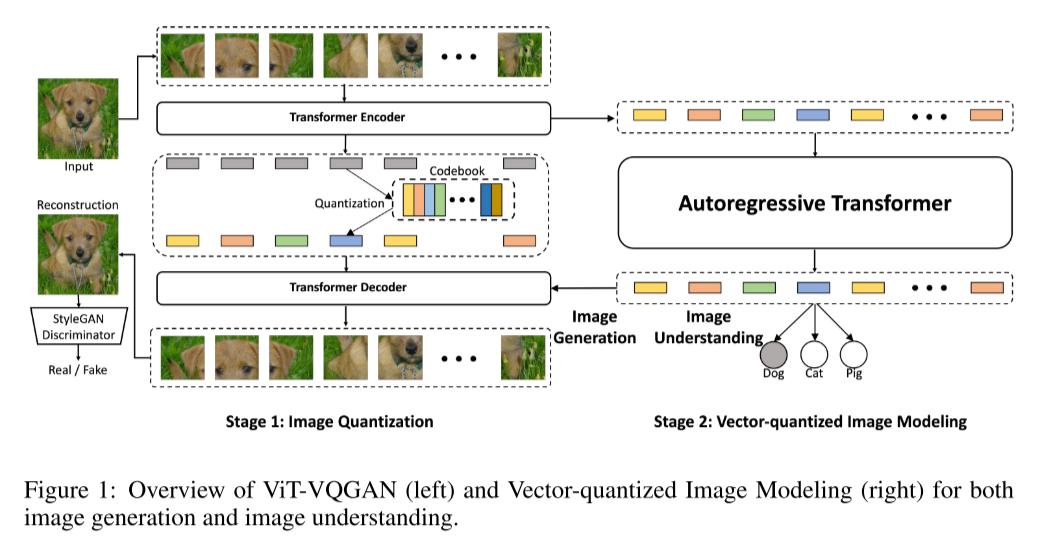
\includegraphics[width=0.8\textwidth]{./fig/ViT-VQGAN.png} 
    %\caption{这是一张示例图片} 
    %\label{fig:example} 
\end{figure}
